%
% CHAPTER Versuch 2
%
\chapter{Abtasttheorem}
Dieser Versuch befasst sich mit dem Abtasttheorem, welches bei der Digitalisierung von Analogen Signalen eine essentielle Rolle spielt.
\label{chap:Abtasttheorem}
\section{Fragestellung, Messprinzip, Aufbau, Messmittel}
\label{chap:VERSUCH_5_FRAGESTELLUNG}
Bei der Digitalisierung von kontinuierlichen Signalen wird in einem gewissen Zeitintervall das Signal abgetastet. Das digitale Signal ergibt sich aus einer Mutliplikation des kontinuierlichen Kurvenverlaufes und der Kammfunktion. Die Abstände der Impulse der Kammfunktion ist gerade die Zeitspanne in der abgetastet wird.
Man kann sich vorstellen, dass bei einer zu geringen Abtastrate Information verloren geht. In der Signaltheorie kann erklärt werden, warum dies der Fall ist. Wie bereits erwähnt kann man die Abtastung einer Funktion(Signal) auch als Multiplikation von Funktion und Kammfunktion darstellen. Die Abtastfrequenz ist gerade die Frequenz der Kammfunktion. Nach der Modulationseigenschaft von Signalen entspricht die Multiplikation der Kammfunktion mit der abzutastenden Funktion einer Faltung der Spektren beider Signale. Das Spektrum der Kammfunktion ist gerade wieder eine Kammfunktion, jedoch mit einer anderen Frequenz. Es gilt also: Je höher die Abtastfrequenz, desto größer die Periodendauer im Spektrum der Kammfunktion und umgekehrt. Wird das Spektrum der zu diskretisierenden Funktion mit der Kammfunktion gefaltet, so wird dieses unendlich oft repliziert. An jedem Impuls ensteht also eine Kopie des Spektrums. Das Spektrum dieser diskreten Funktion ist nach der Abtastung periodisch. Die Periodendauer des Spektrums hängt von der Abtastfrequenz ab. Bei kleinerer Abtastzeit wird die Periode des Spektrums im diskretisierten Signal größer und umgekehrt. Die Spektren rücken also je nach Abtastfrequenz näher zusammen oder weiter auseinander. 
Wird zu gering abgetastet überlappen sich die Spektren und das Originalsignal kann nicht mehr verlustfrei hergestellt werden. Dieses Phänomen nennt sich auch Aliasing. Damit kein Aliasing auftritt muss man beachten, dass ausreichend hoch abgetastet wird. Die minimale Abtastfrequenz ist gerade die doppelte Maximalfrequenz des Signals und nennt sich Nyquistfrequenz. Hält man bei der Abtastung die Nyquistfrequenz ein kommt es zu keinem Aliasing. 
Das Abtasttheorem besagt also, dass ein auf $fmax$ bandbegrenztes Signal mit einer Frequenz von größer $2 \cdot fmax$ abgetastet werden muss, damit man es aus dem zeitdiskreten Signal wieder exakt rekonstruieren kann.
In diesem Versuch wird ein Sinussignal von der halben Nyquistfrequenz bis hin zur Abtastfrequenz erhöht um zu sehen, was dies für Auswirkungen hat.
Die Abtastfrequenz des AD-Wandlers beträgt 80000$Hz$. Die Nyquistfrequenz beträgt somit genau 4$kHz$. Die Frequenz des Signals wird in sieben Schritten erhöht. Die entsprechenden Spektren sind folgen zu sehen.

\section{Messwerte}
\label{chap:VERSUCH_5_MESSWERTE}

\begin{figure}[H]
\centering
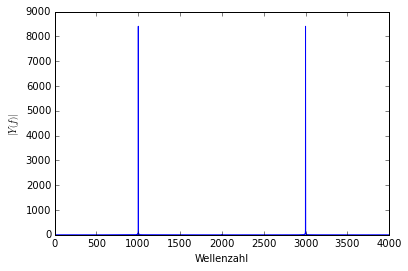
\includegraphics[width=0.75\textwidth]{5_2000.png}
\caption{Frequenzbereich 2kHz}
\label{fig:F2}
\end{figure}
\begin{figure}[H]
\centering
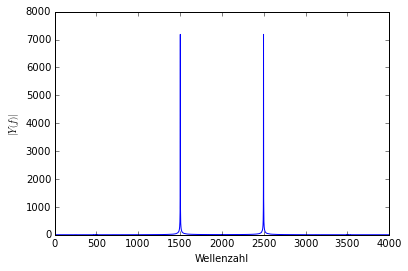
\includegraphics[width=0.75\textwidth]{5_3000.png}
\caption{Frequenzbereich 3kHz}
\label{fig:F3}
\end{figure}
\begin{figure}[H]
\centering
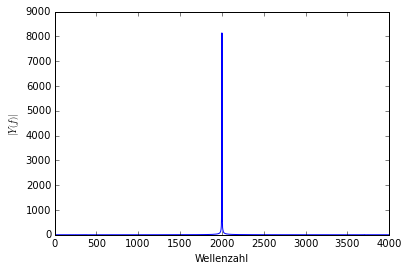
\includegraphics[width=0.75\textwidth]{5_4000.png}
\caption{Frequenzbereich 4kHz}
\label{fig:F4}
\end{figure}
\begin{figure}[H]
\centering
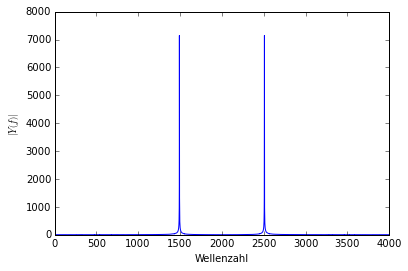
\includegraphics[width=0.75\textwidth]{5_5000.png}
\caption{Frequenzbereich 5kHz}
\label{fig:F5}
\end{figure}
\begin{figure}[H]
\centering
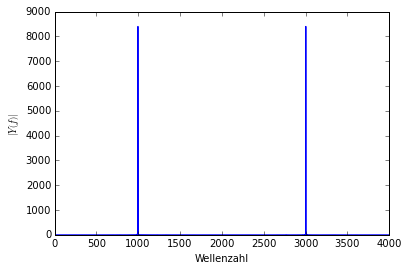
\includegraphics[width=0.75\textwidth]{5_6000.png}
\caption{Frequenzbereich 6kHz}
\label{fig:F6}
\end{figure}
\begin{figure}[H]
\centering
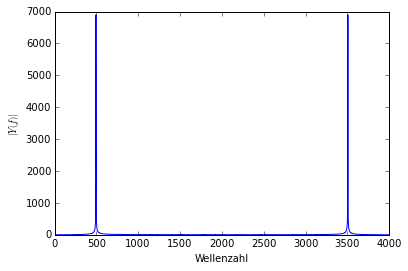
\includegraphics[width=0.75\textwidth]{5_7000.png}
\caption{Frequenzbereich 7kHz}
\label{fig:F7}
\end{figure}
\begin{figure}[H]
\centering
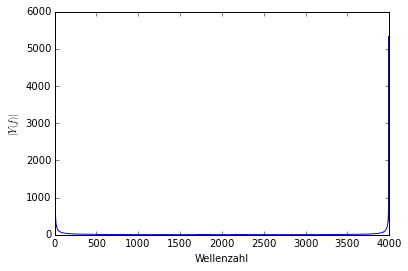
\includegraphics[width=0.75\textwidth]{5_8000.png}
\caption{Frequenzbereich 8kHz}
\label{fig:F8}
\end{figure}

\newpage
\section{Auswertung und Interpretation}
\label{chap:V5_AUSWERTUNGUNDINTERPRETATION5}
Auf der x-Achse ist die jeweilige Wellenzahl aufgetragen. Die entsprechenden Frequenzen stehen unterhalb der Grafik. In Abbildung \ref{fig:F2} ist das Spektrum einer Sinusschwinung mit 2000Hz zu sehen. Dies entspricht dem Impuls bei der Wellenzahl 1000. Der andere Impuls bei Wellenzahl 3000 ist bereits die Nächste Periode im Spektrum. Er ist quasi eine Kopie des Spektrums bei Wellenzahl 1000. In diesem Fall liegt die Maximalfrequenz des Signals unterhalb der Nyquistfrequenz des AD-Wandlers und es kommt nicht zu Aliasing.
In der nächsten Abbildung wurde die Frequenz der Sinusschwinung erhöht, was ein zusammenrücken der Spektren zufolge hat. Auch nun überlappen sich die Signale in der Fourierdomäne noch nicht, da die Frequenz der Schwinung noch unterhalb der Nyquistfrequenz liegt.
In der nächsten Abbildung liegen die Spektren genau übereinander, denn die Frequenz der Sinusschwinung ist gerade die Nyquistfrequenz. Obwohl sich die Spektren genau überlappen könnte man nun noch das Signal wiederherstellen, da die halbe Abtastfrequenz gleich und nicht kleiner als die maximale Frequenz der Sinusschwinung ist. 
In Abbildung \ref{fig:F5} sind die Spektren aneinander vorbeigelaufen. Sie überlappen sich also und Aliasing kommt zum vollen Zuge, da die Frequenz der angelegten Sinusschwinung nun größer als die halbe Abtastfrequenz ist. Das Originalsignal kann nun nicht mehr ohne weiteres Verlustfrei hergestellt werden. Es schleichen sich Frequenzen ein, die im Ursprünglichen Signal gar nicht vorhanden waren.
Der Impuls bei Wellenzahl 2500 repräsentiert die Schwingung mit 5000Hz.  Der Impuls bei Wellenzahl 1500 ist eine neu hinzugekommene Schwingung, die im Originalsignal nicht vorhanden war.
In den weiteren Abbildungen ist zu sehen, wie die Impulse immer weiter auseinanderrücken. Würde man die Frequenz weiterhin erhöhen müsste nach dem letzten Bild wieder ein neuer Impuls einer anderen Periode des Spektrums ins Bild rücken.
 